% GUID v7: From Inflation to the Standard Model, read through the axioms of DMP. Draft of 4 November 2026.
% Build: pdflatex guid-v7.tex twice (bibliography inline). Checks: python3 checks.py (60 checks). Run record: runs/ (de/, pt/, bh/).
\documentclass[11pt,a4paper]{article}
\usepackage[T1]{fontenc}
\usepackage[utf8]{inputenc}
\usepackage{lmodern}
\usepackage[margin=2.5cm]{geometry}
\usepackage{amsmath,amssymb}
\usepackage{booktabs,tabularx,array,longtable}
\usepackage{enumitem}
\usepackage{graphicx}
\usepackage[hidelinks]{hyperref}
\usepackage{url}
\setlength{\emergencystretch}{3em}
\newcolumntype{L}{>{\raggedright\arraybackslash}X}
\newcommand{\chk}[1]{\textsf{[#1]}}
\newenvironment{erabox}{\par\smallskip\noindent\tabularx{\linewidth}{@{}>{\bfseries}p{1.6cm}L@{}}\toprule}{\bottomrule\endtabularx\par\smallskip}

\title{GUID v7: From Inflation to the Standard Model,\\ read through the axioms of DMP\\[0.6ex]
\large One timeline from the end of inflation to today's accelerating expansion, with its black holes, its matter surplus, its
particles and its dark energy, tested on data and on the lattice}
\author{Steven Hrovat\thanks{Independent. Contact: \href{mailto:hrovat.steven@googlemail.com}{\nolinkurl{hrovat.steven@googlemail.com}}.}
\and Sirius (Claude, Anthropic)\thanks{An AI system working as the coordinator of the first author's projects. See ``Contributions and use of AI''.}}
\date{Draft of 4 November 2026}

\begin{document}
\maketitle

\begin{abstract}
\noindent GUID reads the Dark Matter Protocol (DMP~0.9.9), an axiom system for trust built on a Duality of two witnesses, as physics. Earlier
stages read single topics. This stage reads one timeline, from the end of inflation to today, and confronts each era with measurement,
with our own simulations, or both. Inflation is Starobinsky's, adopted from physics; a lattice run shows it does not fragment, so the
oscillon route of v6 is dropped. A rollout principle agreed with the first author (``the most stable state possible \dots by the most efficient
path available within the time the expansion allows'') makes a hidden switch lag at $10^5$--$2\times10^7$~GeV; its lagging patches can collapse to
asteroid-mass black holes that are not excluded as all of the dark matter, in the window $2\times10^{17}$--$10^{22}$~g, but only if the switch
decays slowly and its speed is tuned, because a 2025 gauge objection kills the fast version. The same event leaves a gravitational-wave hum
at 0.02--0.7~Hz and, through an
out-of-balance decay, the matter surplus; the ratio of dark matter to ordinary matter then depends on one number, a mirror preference
of about $10^{-8}$ per decay, which the axioms do not yet supply. Neutrinos are taken as Majorana. In the particle sector a balance rule
fuzzed over 696 forms beats chance only for the charged leptons (the Koide relation), and a laptop lattice of pure gluons and quenched
quarks reproduces confinement, the first-order deconfinement of three colours, the topological susceptibility, the $\eta'$ mass
($963\pm37$~MeV) and, after a three-spacing continuum extrapolation, the nucleon--$\Delta$ spin gap. For dark energy the first author's
picture, space made by the uncaptured leftovers of weak interactions and slowed as matter clumps, fits the expansion history of DESI DR2, two
supernova samples and Planck about as well as DESI's $w_0$--$w_a$ form with no continuous shape parameter (the act type and one mass scale were
chosen from a scan); after trials this is a 1--2$\sigma$ preference over a constant. It predicts a peak near redshift 0.5, a steep fall before
it, and $S_8\approx0.85$, which is 3.7--5$\sigma$ above DES six-year lensing; with lensing included the law is level with or behind the
constant. Its amount is not derived. One script of 60 checks re-derives the quoted numbers.
We claim that the timeline is coherent where stated and that it breaks where stated, not that it is correct.
\end{abstract}

\noindent\textbf{Keywords.} Starobinsky inflation; supercooled phase transition; primordial black holes; gravitational-wave background;
baryogenesis; Majorana neutrinos; Koide relation; lattice QCD; emergent space; dynamical dark energy; DESI.

\tableofcontents
\bigskip

\section{Introduction}\label{sec:intro}

GUID is the name of a series of papers that read an axiom system for trust, the Dark Matter Protocol~\cite{dmp}, as physics. The series
has one standing verdict: DMP \emph{cannot model} quantum gravity in our universe but \emph{can host} it as content. That is why the title says
``read through'', not ``modelled by''. A reading takes a structure the axioms impose and asks whether nature has the same structure; it
does not derive numbers the axioms do not contain. Where the axioms are silent we adopt physics, say so, and test the whole.

Earlier stages read single topics: gravity and the fine-structure constant, the balanced state, the vector and scalar fields. Version~6
stated, simulated, tested and judged 72 confrontations and found that all three GUID-specific claims reachable by data failed. This stage
does something different. It asks the first author's question directly: does one timeline, from the end of inflation to the accelerating
universe of today, hang together when every era is read through the axioms, and where does it break? It is an exploration, run on the
first author's laptop (a lattice code on an 8~GB GPU), in a cloud session (data fits), and in a parallel black-hole work package. The
first author steers by ideas and judgement; the models translate them into mathematics and test them. Where a step depended on his choice we
quote it with its time (UTC, 1--4 November 2026).

\paragraph{How to read the boxes.} Each era ends in a box with four lines: \textbf{holds} (agrees with measurement or with an established
result), \textbf{reading} (a correspondence between the axioms and known physics that adds no number), \textbf{open} (a gap), and
\textbf{test} (the measurement that decides it). Section~\ref{sec:ledger} collects them.

\paragraph{What changed from v6.} (1) The oscillon route to dark matter is dropped (Section~\ref{sec:inflation}). (2) A lagging switch
supplies black holes, a hum and the matter surplus (Sections~\ref{sec:switch}--\ref{sec:surplus}). (3) Neutrinos are Majorana, not Dirac
(Section~\ref{sec:neutrinos}). (4) The particle sector is tested by fuzzing and by lattice simulation (Sections~\ref{sec:ew}--\ref{sec:hadrons}).
(5) Dark energy, absent from every earlier stage, gets a law and a fit (Section~\ref{sec:de}). Version~6 stays as it is.

\section{The axioms and the rules of reading}\label{sec:axioms}

\subsection{The three axioms and the ground}
DMP~0.9.9~\cite{dmp} has three axioms. \emph{Axiom~1, the Duality}: a part acts only while two independent witnesses, one owning trust
and one owning information, each with full reach and gated only by the other, trust it for that act; neither overrules the other, and
the balance is the direction of the system. \emph{Axiom~2, Trust}: trust is gravitational, a field and never a position, with a source,
a depth and a freshness that decays; a strong enough boundary contains, and what still leaves is entropy. \emph{Axiom~3, Information}:
every act leaves a record that its witnesses can read in full and that outlives the act; any other reader sees the counts always and the
content only by a grant. Everything rests on a ground, G0, ``stated, not derived''. As in the earlier stages, trust is read as existence,
the trust half as a classical existence field spanning 3+1 dimensions, and the information half as a scalar that sets the fine-structure
constant and carries quantum content.

\subsection{Rules this stage adds}
Three rules were agreed with the first author during the exploration. They are readings, not theorems of DMP.

\paragraph{The rollout principle} (agreed 1~Nov, 10:34Z, after a proposed amendment). ``Once any building block is possible, the most
stable state possible is always optimized for as efficiently as possible, by the most efficient path available within the time the
expansion allows. So once any force split is possible, that is the new most efficient path; where that path has a barrier, the switch lags,
and the patches it leaves behind are excluded.'' His first form had no clause about time; strictly read it forbids supercooling, freeze-out
and the metastable Higgs vacuum, all of which nature shows, so the clause was added. ``Excluded'' means, in his words, ``no act can carry
over, but they still bend the same relativistic plane'': behind a horizon, still gravitating.

\paragraph{Shape and counts} (1~Nov, 14:08Z--14:11Z). ``Since it goes towards the most efficient assertion of Existence, and Existence in
the universe is defined as 3s1t, those are the parts to optimize for.'' Tested, this holds for \emph{shape} (handedness exists only in even
spacetime dimensions; SU(2) is the double cover of rotations of three axes; stable orbits and atoms exist only in three space dimensions
\cite{ehrenfest,tegmark}) and fails for \emph{counts} (three pions for two light flavours, eight gluons). The accepted form is: \emph{3s1t sets
the shape, the balance sets the counts.}

\paragraph{Continuous balance} (14:06Z). ``The balanced state is and always be continuous, since a single point would mean total absence of
possible change and no causality.'' A continuous family of balanced states is what, in field theory, produces massless Goldstone modes;
this is the reading used for the pion (Section~\ref{sec:hadrons}).

\subsection{Method}
Inputs are standard values (PDG, Planck, published fits) unless a number is ours. Each external number in the notes carries its source
and the date read, or is marked ``from memory''; the latter are flagged where they matter. Every scan keeps its count of forms tried, and a
fit counts only if it beats a null or predicts something it was not fitted to. The 60 checks in Appendix~\ref{app:checks} re-derive the
analytic numbers and re-read the fitted ones from the run outputs.

\section{Inflation}\label{sec:inflation}

GUID's own hypothesis for the start places no restriction on geometry inside it~\cite{guidv6}; the inflaton is not GUID's. We adopt
Starobinsky's $R^2$ inflation~\cite{starobinsky}, the best-fitting plateau model, with $n_s=1-2/N$ and $r\approx3\times10^{-3}$, as v6 did.
The first author reads inflation through his Oscillon Degradation Protocol: ``very fast exploration, then abrupt setting of the boundary,
then slow rolling out'', which maps onto inflation, its end, and reheating with bubble percolation.

\paragraph{No oscillon era.} Version~6 named oscillons, long-lived lumps of the inflaton, as the seed of black-hole dark matter. Two results
end that route. First, a mass-scale argument: black holes in the asteroid window need a Hubble rate of at most $\sim10^{-3}$~GeV when they collapse
(at most about 1~GeV at the end of inflation, allowing for growth of the lumps), while Starobinsky inflation has $H\sim10^{13}$~GeV, so its oscillons would make gram-scale holes that evaporate at once; Cotner, Kusenko and
Takhistov say so for their own model~\cite{cotner2018}. Second, a direct lattice run of the Starobinsky potential with vacuum initial
fluctuations and nothing tuned (256$^3$, scale factor to 18) shows no fragmentation at all: the largest density contrast stays at
$1.0003$ in every snapshot, as Lozanov and Amin's criterion predicts for potentials that flatten at the Planck scale~\cite{lozanov}. A
monomial scan that seemed to give the needed few thousand lumps per horizon did not converge with resolution and was withdrawn. The
information scalar as a spectator field also fails: if it decays only through its coupling to light, the lumps decay after nucleosynthesis
even when $\alpha$ is allowed to swing between 1 and 1/128 (60 times short in coupling). On 1~Nov at 10:11Z the first author decided:
adopt Starobinsky and drop the oscillon route (``our model generally doesn't go the oscillon route'').

\paragraph{The tilt.} With the switch of Section~\ref{sec:switch} the slow-decay matter era removes about one e-fold, giving
$n_s=0.963$--$0.966$ and $r=0.003$--$0.004$: inside Planck's $0.9649\pm0.0042$~\cite{planck}, but ACT DR6 with Planck and DESI prefers
$n_s\approx0.974\pm0.003$~\cite{act}, which puts Starobinsky at 2--3$\sigma$; our matter era makes it slightly worse. A stiff phase cannot add
the needed $\sim17$ e-folds. This is external to GUID: later eras need from inflation only a reheating temperature above about
$3\times10^7$~GeV (Starobinsky gives $2.3\times10^9$~GeV through gravitational decay to the Higgs) and the measured large-scale ripples.

\begin{erabox}
holds & Starobinsky fits Planck; it does not fragment (our lattice, consistent with Lozanov--Amin). \\
reading & ODP's exploration, boundary and rollout = inflation, its end, reheating with percolation. \\
open & ACT's $n_s\approx0.974$ (2--3$\sigma$); a modified $R^2$ model would be adopted, not derived. \\
test & Simons Observatory, CMB-S4 ($n_s$, $r\approx0.003$). \\
\end{erabox}

\section{The switch}\label{sec:switch}

\paragraph{The idea.} On 1~Nov at 10:11Z the first author proposed that $\alpha$ is the \emph{binding} of existence and information, that
is, how strongly the SU(2) field $W^3$ and hypercharge $B$ are bound (textbook: the mixing angle, $1/\alpha=1/\alpha_W+1/\alpha_Y$), and that
at a rapid change ``sweet-spot'' regions bind and stay while the rest passes them; a few bubbles remain and build up. In physics this is a
first-order phase transition with delayed regions: the last patches to switch keep vacuum energy and can collapse~\cite{liu2021,baker2021,
kawana,gouttenoire,lewicki}. The Standard Model's own electroweak transition at 160~GeV is a crossover with no bubbles, and its horizon mass
($\sim10^{28}$~g) is excluded as all of the dark matter, so the switch must be new and sit at $T\approx10^5$--$2\times10^7$~GeV (the light edge, $10^{17}$~g, is excluded).

\paragraph{The field.} The best match is a classically conformal dark U(1)$_X$ whose only link to us is kinetic mixing,
$\epsilon\,X_{\mu\nu}B^{\mu\nu}$, the unique renormalisable vector portal, touching hypercharge and never $W$~\cite{aixie}. Its Coleman--Weinberg
potential supercools deeply, so the switch is a brief vacuum-dominated phase, abrupt percolation, then slow decay of the field: the start's
pattern repeated one layer down. In the reading, $\epsilon$ is the binding strength of the hidden sector into ours. Ruled out as the switch:
the information scalar itself (no potential, frozen in the plasma: in radiation $\langle E^2-B^2\rangle\approx0$ does not drive it), the
Higgs (crossover), a conformal B$-$L field (it would fix the neutrino character before we chose it), and the axion (QCD scale,
solar masses).

\paragraph{Slowest rollout.} The first author asked for the ``slowest rollout possible''. As a \emph{sequence} of steps it holds. As the speed
of one switch it overshoots. In the slow-decay version that survives (Section~\ref{sec:bh}) all of the dark matter needs $\beta/H\approx9.5$--$14.6$
and a slower switch makes more black holes, so ``slowest'' overproduces; the superseded fast-reheating fit showed the same ($7\times10^{11}$ times
the dark matter at $\beta/H=3$ for $10^{19}$~g). Below $\beta/H\approx3$ bubbles never percolate; for conformal potentials a lower bound near 5 has
been given~\cite{confbound}. The agreed form is ``longest sequence, each step as fast as its
own physics allows''. The rate $\beta/H$ is the one knob GUID does not fix.

\begin{erabox}
holds & A supercooled conformal U(1) gives the vacuum-dominated phase, abrupt percolation and slow decay (literature). \\
reading & Delayed patches are overdense, qualitatively only (our lattice: last 5\% of blocks $+0.2$ to $+5.6$, flat slicing, not converged at the walls, gauge dependent, \S\ref{sec:bh}). Lag = barrier on the most efficient path; excluded patches = collapse behind a horizon; $\epsilon$ = binding into $B$. \\
open & $\beta/H$; whether the hidden field has any tie to the information scalar. \\
test & The hum (Section~\ref{sec:bh}); a dark photon at $10^7$--$10^8$~GeV is beyond colliders. \\
\end{erabox}

\section{Black holes as the dark matter}\label{sec:bh}

The asteroid-mass window, about $10^{17}$--$10^{22}$~g, is the one mass range where primordial black holes can still be all of the dark
matter~\cite{gortongreen}. A hole of mass $M$ forms near horizon entry at $t\approx GM/c^3$: $2.5\times10^{-22}$~s for $10^{17}$~g and
$2.5\times10^{-17}$~s for $10^{22}$~g, when the plasma was at $3\times10^7$ to $10^5$~GeV \chk{A10}. The whole window lies inside the
symmetric electroweak era, far before quarks bind. Version~6 already reads a black hole as the contained remnant: a containing boundary is
an event horizon, and outside it only mass, spin and charge are counted (Axiom~3's counts).

A five-part work package tested the lagging switch as the source; we summarise its verdict~\cite{wpbh}.

\paragraph{Collapse thresholds.} A Misner--Sharp code (comoving slicing, regular centre, artificial viscosity fixed in advance) reproduces
the radiation-era thresholds of Escriv\`a, Germani and Sheth~\cite{escriva}, $\delta_c=0.4668/0.4978/0.5536$ for profile sharpness
$q=0.5/1/3$ against analytic $0.4569/0.4892/0.5532$, stable to $5\times10^{-4}$ under resolution and boundary changes. With a soft equation
of state the threshold falls (at $w=0.05$, $\delta_c\approx0.19$), and during the slow decay of the switch field it falls to about 0.02--0.08.
Caveat: for the soft profiles ($q=0.5$, 1) these low values are \emph{dispersal boundaries}: a dust-like central singularity forms before any
horizon and the code cannot follow past it; only $q=3$ forms an apparent horizon (constraint error 0.1--0.2). That collapse ends in a black hole
for the profiles that set the numbers is therefore not shown. An earlier collapse code of our own failed its validation and was not used.

\paragraph{The gauge objection decides the radiation era.} Franciolini and co-workers showed in 2025 that the overdensity of a late patch
is about ten times smaller in comoving gauge than in the flat gauge earlier estimates used~\cite{franciolini}. We reproduced their factors
($10$, $4$, $9/4$) from linear theory and built our own spherical model of a patch held in the false vacuum: followed with the full
equations, the needed flat-gauge contrast is 10 to 22 and $\ln P\le-158$ at every $\beta/H\ge4$. With fast reheating there is no
black-hole dark matter. A direct Monte Carlo in flat slicing had shown far more overdense patches than the separate-universe shortcut,
which is exactly why the choice of slicing matters.

\paragraph{The slow-decay rescue works.} If the switch field decays slowly, the universe passes through an early matter era in which
collapse is easy~\cite{aixie,harada2016}. Reproducing Ai and Xie's benchmarks (minimum mass, abundance coefficient, reheating temperature
$0.640\,(\Gamma/H_*)^{1/2}T_V$), all of the dark matter needs $\beta/H\approx9.5$ (decay rate $\Gamma/H_*=3\times10^{-3}$) to $14.6$
($3\times10^{-4}$); $f=1$ is reached by choosing $\beta/H$, so it is reproduced by construction, not predicted. In the reading, the slow decay \emph{is} the lag of the rollout principle. Caveat: two estimators of the matter-era
collapse probability differ by tens in $\ln P$; the problem has moved from ``too few'' to ``how many exactly''.

\paragraph{Window, hum and the one-event test.} With current limits the allowed window is $2.0\times10^{17}$--$9.8\times10^{21}$~g;
$10^{17}$~g is now excluded by evaporation limits and $10^{22}$~g sits at the microlensing edge. The bubble collisions leave a
gravitational-wave hum, diluted by the matter era: inside the allowed $10^{18}$--$10^{21}$~g it lies at 0.022--0.74~Hz with
$\Omega h^2\approx1.6\times10^{-11}$--$1.8\times10^{-10}$ \chk{F} (0.006--2.4~Hz if the excluded edges are included):
DECIGO and BBO hear every case, LISA the heavy end, the Einstein Telescope and Cosmic Explorer the light end, and LIGO--Virgo--KAGRA's third
run sees nothing, as expected. The test we designed reads three things off one event: black-hole mass gives the switch temperature,
the hum's pitch and loudness give $\beta/H$ and $\Gamma/H_*$, and then ``all of the dark matter'' must follow. It cannot fail yet: the
abundance goes as $e^{10\,\beta/H}$, so $\beta/H$ must be known to 2\% while model systematics move the prediction by up to ten orders of
magnitude. One corner is decisive: heavy holes ($\sim10^{21}$~g) with the slowest decay ($\Gamma/H_*=3\times10^{-4}$), where 20\%
suffices and the hum at 0.022~Hz, $\Omega h^2\approx1.9\times10^{-11}$, is in LISA's band.

\begin{erabox}
holds & Window open ($2\times10^{17}$--$10^{22}$~g); the hum is below current limits. Not excluded: slow-decay collapse gives all the dark matter if $\beta/H$ is tuned to 9.5--14.6. \\
reading & The black holes are the contained remnant of the rollout: excluded from causality, still bending spacetime. \\
open & Whether soft-profile collapse ends in a black hole (dispersal boundaries); the two matter-era estimators; non-sphericity; the fast-reheating version is dead. \\
test & Microlensing and 511~keV limits on the window; the hum (LISA, DECIGO, BBO, ET, CE); the heavy corner with LISA. \\
\end{erabox}

\section{The matter surplus}\label{sec:surplus}

Equilibrium erases any asymmetry between matter and antimatter, so a surplus needs an out-of-balance phase; the Standard Model's own
CP violation is about $10^{10}$ too weak at high temperature. The first author's ``weak preference = least-resistance balance'' holds as a
direction, but needs the lag. The black holes themselves cannot make it: holes above $10^{17}$~g do not evaporate, and black-hole
baryogenesis needs holes below $10^9$~g. The coherent version is \emph{cogenesis}: the switch field decays out of equilibrium while
sphalerons are active ($T_{\rm reh}=2\times10^3$--$10^6$~GeV), a fraction $\epsilon$ of decays prefers matter, and 28/79 of the B$-$L
asymmetry ends as baryons.

A Boltzmann integration confirms to all printed digits that
\begin{equation}
\frac{\Omega_{\rm PBH}}{\Omega_b}=\frac{79}{28}\,\frac{\beta_0\,m_X}{\epsilon\,m_p},
\end{equation}
independent of the decay rate: the matter era dilutes black holes and baryons equally. So the observed ratio 5.4 does not depend on the
dilution, only on the event. It fixes $\epsilon/\beta_0=1.8\times10^6$ at $m_X=3.2\times10^6$~GeV \chk{A9} (we take the switch-field mass equal to the switch
temperature, $m_X=T_V$, as the work package does); with the black-hole fraction
$\beta_0$ set by the abundance, the mirror preference needed is $\epsilon\approx5\times10^{-9}$ (fast end of the decay range) to
$1.5\times10^{-8}$ (slow end), independent of the black-hole mass. The baryon density then comes out right: $\Gamma/H_*=3\times10^{-3}$ with
$\epsilon=5\times10^{-9}$ gives $Y_B=9.0\times10^{-11}$ against $8.7\times10^{-11}$ observed.

So 5.4 is not predicted. It fixes one number that GUID would have to supply. Laboratory CP asymmetries are larger ($\epsilon_K=2.2\times10^{-3}$);
$\alpha^4=2.8\times10^{-9}$ is nearby, which is numerology until derived. The electron electric dipole moment probes such a sector at one
loop up to about $10^5$~GeV today and $10^6$~GeV with a hundredfold improvement, depending on how the mixing reaches the electron.

\begin{erabox}
holds & Dilution cancels in $\Omega_{\rm PBH}/\Omega_b$; $Y_B$ comes out at the observed value for $\epsilon\approx5\times10^{-9}$. \\
reading & The surplus is the out-of-balance lag's second leftover; ``least resistance'' gives the direction. \\
open & $\epsilon\approx10^{-8}$ from the axioms (the highest-weight open item of this paper). \\
test & The three-way cross-check (mass, hum, ratio); electron EDM. \\
\end{erabox}

\section{Neutrinos: Majorana}\label{sec:neutrinos}

Version~6 chose Dirac neutrinos. The question matters here because a Majorana neutrino can carry the lepton-number violation the surplus
uses. With heavy partners $N$ at the switch scale, the seesaw $m_\nu=y^2v^2/M$ needs Yukawas of $4\times10^{-5}$ ($M=10^6$~GeV) to
$1.3\times10^{-4}$ ($10^7$~GeV) \chk{A8}, between the electron's $2.9\times10^{-6}$ and the muon's $6.1\times10^{-4}$: no new tiny number,
where Dirac masses need $\sim10^{-12}$. On 1~Nov at 18:38Z the first author decided: ``I would go toward Majorana as well, so let's go that
way.'' His economy reading (two states instead of four) is a reading, not a derivation.

\paragraph{The cost.} If the surplus comes from decays of the heavy $N$ themselves, the Davidson--Ibarra bound~\cite{davidson} allows at most
$\epsilon=10^{-10}$ to $10^{-9}$ at those masses \chk{A8}, short of the needed $5\times10^{-9}$--$1.5\times10^{-8}$ by 5 to 150 \chk{A13}. Two ways out:
two nearly degenerate $N$, where the resonant enhancement~\cite{pilaftsis} needs a mass split of about 1--20\% (a mild near-degeneracy,
our estimate, scaled as the inverse of the shortfall, not computed in full), or the asymmetry made by the switch field directly. On 4~Nov the first author asked whether the
switch-era Majorana neutrino is among the leftovers that drive dark energy (Section~\ref{sec:de}); it is not, because supernova cores at
$\sim30$~MeV cannot make $N$ at $10^6$~GeV, and he withdrew it.

\paragraph{The neutrino balance.} The same balance rule that holds for charged leptons (Section~\ref{sec:ew}) fixes the neutrino masses if one
square root is taken negative, Brannen's form~\cite{brannen}: normal ordering, $m=0.36$, $8.6$, $50.1$~meV, sum $59.1$~meV \chk{A2}, just above the oscillation floor of
$58.7$~meV; inverted ordering would give 102.6~meV, disfavoured by cosmology in $\Lambda$CDM (sum below about 64~meV) but not excluded if dark energy
evolves, as Section~\ref{sec:de} proposes (the bound then relaxes to roughly 0.14--0.16~eV). The sign is a choice, not derived. If Majorana, the
effective mass for neutrinoless double-beta decay is $m_{\beta\beta}=1.2$--$3.9$~meV across the Majorana phases, below the next generation's reach (about
10--20~meV): balance predicts no signal there in the coming decade.

\begin{erabox}
holds & Seesaw at the switch scale needs no new tiny number; the neutrino balance gives a sum (59.1~meV) allowed by cosmology. \\
reading & Majorana as the economical choice (first author's decision). \\
open & A resonant pair or direct decay to reach $\epsilon\sim10^{-8}$; washout by the $N$ (Section~\ref{sec:timeline}); the negative root. \\
test & JUNO and DUNE (ordering); cosmology (a sum below 58.7~meV would break normal ordering itself); no $0\nu\beta\beta$ signal above $\sim4$~meV. \\
\end{erabox}

\section{The electroweak split and the lepton balance}\label{sec:ew}

\paragraph{Before the split.} Above $\sim160$~GeV the Higgs field sits at zero and only thermal masses exist; the photon is born at the
split as $A=\sin\theta_W W^3+\cos\theta_W B$, with $\alpha$ near 1/128. Version~6's information scalar multiplies only the Maxwell term, so
before the split it has nowhere to act. A gauge-invariant extension must put it on $B_{\mu\nu}B^{\mu\nu}$, on $W^aW^a$, or on both; the choice is
new content with a later signature (on $B$ only, the ratio $m_W/m_Z$ would drift with $\alpha$). Either way the scalar is frozen in the
radiation plasma. The first author's ``$\alpha$ anywhere between 1 and 1/128'' in the symmetric era conflicts with the Standard Model's running
($1/\alpha\approx105$ even at the Planck energy); we record it as open.

\paragraph{Fuzzing balance.} The first author asked us to ``fuzz the possibilities'': no hard numbers are given except balance, so try the forms
balance could take and see what fits. Round~1 tried 696 rules (Koide-type sums, mixing angles as powers of mass ratios, ladders, angles) on
three mass schemes against 20\,000 random universes each. Everything is at chance except one: the charged-lepton relation of
Koide~\cite{koide}, $Q=(m_e+m_\mu+m_\tau)/(\sqrt{m_e}+\sqrt{m_\mu}+\sqrt{m_\tau})^2=0.666661$ against $2/3$ with PDG~2022's $m_\tau=1776.86$~MeV
(0.6666645 with PDG~2024's 1776.93) \chk{A1}, look-elsewhere
probability 0.7\%, with the 1981 prediction of the $\tau$ mass behind it. In geometric form the angle is $45^\circ$: the part the three
masses share equals the part that distinguishes them. That is a balance. It fails for quarks ($51.2^\circ$, $47.5^\circ$) and for masses
run to the $Z$ scale. Round~2: it holds only for today's physical masses (the unbroken-era Yukawas miss by $10^{-3}$); the best of 125
colour patterns relating quarks to leptons of their generation is Georgi and Jarlskog's (3, 1/3, 1)~\cite{gj}, best at $10^{7.2}$~GeV within
10\%, chance 3.3\%, in the same era as the switch, noticed after the fact. Reading: balance holds for what can be observed alone.

\paragraph{Counts.} An $n$-node cluster has $n^2-1$ internal moves once the whole-cluster mode is removed: eight gluons for three colours (no
singlet gluon, so no long-range strong force), three or eight light Goldstone mesons, and the whole-cluster mode as the heavy $\eta'$.
Hypercharge is the traceless balance mode between the three-cluster (colour) and the two-cluster (weak): the Standard Model's gauge group
is $S(U(3)\times U(2))$. These are readings of known group theory, not derivations.

\begin{erabox}
holds & Lepton balance (Koide) beats chance (0.7\%); 695 other forms do not. \\
reading & ``Balance holds for what is observed alone''; $n^2-1$ counts; hypercharge as the balance mode; Georgi--Jarlskog near the switch era (post hoc). \\
open & Why the lepton balance is exact today and quarks miss it; how the information scalar couples before the split; $\alpha$ before the split. \\
test & Any improved $\tau$ mass (Koide predicts $1776.97$~MeV); $m_W/m_Z$ drift with $\alpha$ if the scalar couples to $B$ only. \\
\end{erabox}

\section{The strong split and the hadrons}\label{sec:hadrons}

This era was tested on the first author's laptop with our own lattice code: SU(3) gauge fields (Cabibbo--Marinari heat bath with
overrelaxation, CUDA, single precision checked against double), then quenched Wilson quarks (even--odd preconditioned BiCGStab with a
single-precision inner solve, Gaussian smearing on APE-smeared links). The pure-gauge plaquette at $\beta=6.0$, $0.59366(1)$, matches the
reference $0.5937$; the quark code passes $\gamma_5$-hermiticity ($4\times10^{-13}$), gauge covariance and the free-field limit.

\subsection{Gluons alone}
\begin{itemize}[leftmargin=*,itemsep=2pt]
\item \textbf{Confinement.} The static potential at $\beta=6.0$ gives $a\sqrt\sigma=0.217(2)$ and $r_0/a=5.30(4)$ (literature 0.22 and, Necco--Sommer, 5.368; the topological susceptibility below
uses 5.37), so $\sqrt\sigma\approx454$~MeV with $r_0=0.5$~fm.
\item \textbf{Deconfinement order.} The Polyakov loop on $12^3\times4$ jumps at $\beta=5.69$ with a double-peaked histogram (literature
$\beta_c=5.6925$), and its susceptibility grows with volume: three colours deconfine with a first-order jump. Two colours (SU(2)) rise
smoothly with no double peak: a continuous transition, as Svetitsky and Yaffe predict from the centre symmetry~\cite{svetitsky}. Reading:
the three-node cluster holds its containment until a sharp break; the two-node cluster softens gradually.
\item \textbf{Mass from gluons alone.} The lightest glueball at $\beta=6.0$ and $5.85$, extrapolated in $a^2$, gives
$m/\sqrt\sigma=3.34\pm0.23$ against $3.405$ from Athenodorou and Teper~\cite{athenodorou}, about 1.5~GeV: mass without any quark mass.
\item \textbf{The strong-CP angle.} With gradient flow on 240 configurations the topological susceptibility is $\chi^{1/4}=179.9\pm4.3$~MeV
(literature 185--191), and the vacuum energy rises as $\chi\theta^2/2$ away from $\theta=0$: the minimum is at zero, as Vafa and Witten
proved~\cite{vafawitten}. Through Witten and Veneziano's relation~\cite{witten,veneziano} our $\chi$ gives $m_{\eta'}=963\pm37$~MeV against
958 measured \chk{A6, A7}. Why nature sits at $\theta=0$ rather than merely could: open (it needs a field that rolls there).
\end{itemize}

\subsection{Quarks: three spacings and the continuum}
With quenched Wilson quarks at four masses per spacing, the pion mass squared falls linearly to zero with the quark mass (fit $\chi^2/{\rm dof}=0.81/2$),
and the partially conserved axial current gives the same critical point to $10^{-4}$: the pion is a Goldstone ripple, which is what the
continuous balance demands. The $\rho$ meson, at $772\pm14$~MeV at one spacing, extrapolates to 836 (in $a^2$) to 914~MeV (in $a$) in the continuum, against 775
measured: heavy, the cost of spin~1, and 8--18\% high like the other masses in MeV. After an
overnight chain lost to a desktop restart was relaunched detached, three spacings were finished ($\beta=5.8$, $6.0$, $6.2$; $a=0.140$, $0.094$,
$0.068$~fm; 100 configurations at the finest). Wilson quarks carry errors linear in $a$, so we extrapolate in $a$ and show $a^2$ as a comparison.
Ratios do not depend on the scale $r_0$:

\begin{center}\small
\begin{tabular}{@{}lccc@{}}
\toprule
ratio & $a\to0$, linear in $a$ & $a\to0$, linear in $a^2$ & measured \\
\midrule
$m_\Delta/m_N$ & $1.28\pm0.08$ & $1.23\pm0.05$ & 1.313 \\
$(m_\Delta-m_N)/m_\rho$ & $0.39\pm0.11$ & $0.33\pm0.06$ & 0.379 \\
$m_N/m_\rho$ & $1.30\pm0.08$ & $1.42\pm0.05$ & 1.21 \\
\bottomrule
\end{tabular}
\end{center}

\noindent In the linear-in-$a$ column the spin gap and the $\Delta/N$ ratio land on the measured values within errors, from gluons and
quenched valence quarks alone; in $a^2$, $\Delta/N$ is 1.7$\sigma$ low, $(\Delta-N)/\rho$ carries a 28\% error in $a$, $m_N/m_\rho$ misses
(1.1 and 4$\sigma$), and the nucleon and $\Delta$ fits have poor $\chi^2$ in both. A weak hold. In MeV the masses come out 6--25\% high and
$f_\pi$ about 9\% high ($142$ against 130~MeV): quenching, the $r_0$ scale and a linear chiral extrapolation from pions of about 620~MeV
and up. $r_0=0.5$~fm is the quenched convention; a phenomenological $r_0$ of 0.47--0.49~fm would raise every MeV value by 2--6\% (so 8--33\%
high); the ratios are unaffected. Caveats: one physical volume (1.5--1.6~fm), and $Z_A$ and $r_0$ taken from memory.

\subsection{Readings of hadron structure}
\begin{itemize}[leftmargin=*,itemsep=2pt]
\item \textbf{The witness rule.} If each quark must be witnessed by the other two (all three colours different), exactly the 56 ground-state
baryon states seen are allowed (octet and decuplet); without it, 20, and no $\Delta^{++}$, which is refuted. This is the colour argument of
Greenberg and of Han and Nambu~\cite{greenberg,hannambu} in the axioms' words, and the strongest reading of this section.
\item \textbf{Spin balance.} Opposite spins are cheaper in 8 of 8 meson pairs and 8 of 8 baryon pairs (chance $4\times10^{-3}$ for the baryons alone), with gaps that
shrink as $1/(m_1m_2)$ for heavier quarks; the lattice spin gap grows toward light quarks at every spacing. This is the standard colour-magnetic
hyperfine force, read as balance.
\item \textbf{The pion's decays.} $\pi^0\to\gamma\gamma$ at a rate set by $\alpha^2$ gives 7.76~eV against 7.8 measured \chk{A3}; this is the
textbook Adler--Bell--Jackiw anomaly, with the three colours entering squared. The first
author's ``a two-node cluster drains, predictable through $\alpha$'' holds for the neutral pion. For the charged pion his ``always the
highest-entropy path'' fails: phase space prefers $e\nu$ by 5.5, but handedness suppresses it by $(m_e/m_\mu)^2$ to $1.283\times10^{-4}$
\chk{A4}; handedness decides first, balance only within what handedness allows. The charged--neutral mass difference from $\alpha$ (Das et
al.~\cite{das}) with the measured $\rho$ mass gives 5.29~MeV against 4.59 \chk{A5}, 14\% high: the right order. With our continuum
$\rho$ it would be 6.1--7.3~MeV.
\item \textbf{Quark--gluon plasma in small systems.} The 2025 oxygen--oxygen runs at the LHC and RHIC show jet suppression in small
systems (CMS: minimum $R_{AA}=0.69\pm0.04$ near 6~GeV~\cite{cmsoo}) and no sign of a size threshold (the crossover temperature of about 156~MeV is a lattice value, not measured in these collisions).
Consistent with the reading of a local balance state, and not able to tell GUID from standard QCD.
\end{itemize}

\begin{erabox}
holds & Confinement, first-order SU(3) vs smooth SU(2), glueball mass, $\eta'$ mass, pion mass squared linear in the quark mass, $\pi^0$ width (the anomaly); continuum spin gap and $\Delta/N$ (weak: quenched, one volume, heavy pions). \\
reading & Witness rule = colour; spin balance = hyperfine force; continuous balance = Goldstone; $\theta$ minimum at 0 reproduces Vafa--Witten; $\pi^\pm-\pi^0$ right in order (14\% high). \\
open & Why $\theta=0$; why exactly the light flavours form a valley; why three generations stop at three. \\
test & Unquenched, larger-volume lattice (not on this laptop); improved $\tau$, $\eta'$, $\theta$ bounds (neutron EDM). \\
\end{erabox}

\section{The whole timeline}\label{sec:timeline}

A single pass over all eras with the v7 parameters: Starobinsky reheats at $2.3\times10^9$~GeV, above the switch \chk{F}; the switch field
decays at $2\times10^3$--$10^6$~GeV, long before nucleosynthesis; sphalerons are active then, so the surplus converts; the hum's energy is far
below the $N_{\rm eff}$ bound; black holes above $10^{17}$~g do not evaporate before today, so nucleosynthesis and the CMB are untouched;
accretion limits on the CMB apply only above about a solar mass; Poisson isocurvature at these masses is negligible; the surplus is
homogeneous. Everything passes, except the CMB tilt (Section~\ref{sec:inflation}), which is external, and dark energy, which was absent from
v7 until the last day and is the subject of the next section.

\paragraph{Not yet checked: washout.} Two eras meet here. With Majorana partners $N$ at $10^6$--$10^7$~GeV and $\tilde m\sim m_{\rm atm}$, the
decay parameter is $K=\tilde m/m_*\sim50$, strong washout. During the slow decay the plasma reaches a maximum temperature of order $0.2\,T_V$,
up to a few $10^6$~GeV, above the final reheating temperature. Inverse decays of $N$ can then erase the B$-$L asymmetry the switch field makes,
unless $M_N$ sits well above that maximum temperature. We have not computed it; it is open (ledger item 54).

\section{Dark energy: the leftover law}\label{sec:de}

\subsection{The question and what was ruled out first}
DESI's second data release, combined with the CMB and supernovae, prefers a dark energy that changes with time over a constant, at
2.8$\sigma$ with Pantheon+, 3.8$\sigma$ with Union3 and 3.2$\sigma$ with DES five-year supernovae after the Dovekie recalibration
(4.2$\sigma$ before it)~\cite{desi,popovic}; its fitted equation of state crosses $w=-1$, which no single canonical
scalar field can do. The first author's idea (4~Nov, 17:20Z): ``the possibility space of Existence growing according to what the current
conditions are. The possibility of something existing there inflating the space, so that there is room for it to.'' Four routes were tested
before his driver.

\begin{itemize}[leftmargin=*,itemsep=2pt]
\item \textbf{The information scalar as dark energy.} Atomic clocks bound its drift so tightly (coupling below $10^{-7}$; v6 already had
$|\lambda|<1.7\times10^{-8}$) that it cannot be the dark energy, and as one scalar it cannot cross $-1$. On 4~Nov at 17:23Z the first author
dropped it: ``Linking it to the information field seems to have no actual basis in science, but the space emergence seems like a good path to
follow.''
\item \textbf{Emergent space.} Padmanabhan~\cite{padmanabhan} writes the growth of cosmic volume as $dV/dt=L_P^2(N_{\rm sur}-N_{\rm bulk})$:
space emerges until the degrees of freedom on the horizon equal those inside, and de~Sitter space is that balance reached. This has the shape
of the first author's idea and is our framework.
\item \textbf{The $4\pi$ rule.} A follow-up postulates that the number of modes crossing the horizon, $N_c=(2/3\pi)\ln[(aH)_{\rm end}/(aH)_{\rm min}]$,
equals $4\pi$, which fixes the cosmological constant. We derived the count ourselves (the source was not readable from our session). With
instant reheating near $10^{15}$~GeV it works ($N_c=12.88$ against $12.57$). With our timeline it fails: Starobinsky's slow reheating gives
11.90 and $\Lambda$ at $10^{-8}$ of observed; the switch's matter era and supercooling push it to 9.5--11.7 and $10^{-11}$ to $10^{-38}$
\chk{F}. Either the rule or the timeline is wrong; they cannot both stand.
\item \textbf{Deformed horizon entropy} (Barrow, Tsallis): these change the whole expansion history, and the deformation DESI would need
is about a hundred times what nucleosynthesis allows.
\end{itemize}

\subsection{The driver, as the first author stated it, and the order of fitting}
Over the next hour he stated and sharpened the driver. The order matters for what the fit is worth, so we state it plainly. The
supernova-rate tracer (leftovers from core-collapse supernovae times the unclumped share) was introduced by us in a scan and fitted to the
full data before his 17:56Z choice of the weak interaction, which he made knowing that it ``lines up with what the data implies''; his
17:31Z statement names neither star formation nor supernovae. The escape mass was scanned over $10^9$--$10^{13}\,M_\odot$ ($\Delta\chi^2$
from $-7.8$ to $+7.8$) and the data chose $10^9$--$10^{10}$. (The headers of the dark-energy note run about one hour ahead of these UTC
times.) The steps:
\begin{enumerate}[leftmargin=*,itemsep=2pt]
\item (17:31Z) ``the pressure generated by the acts asserting Existence, which inflate the Existence Space, being slowed down by the clumping
together of Existence and the strong associated gravitational pull \dots\ as everything clumps back together, even the evidence of acts no
longer leave the local area, thus stagnating.''
\item (17:49Z) Acts follow matter evenly; dark matter adds to the clumping but not the acts. \emph{Refuted}: a steady act rate never turns over,
and every form is worse than a constant by 11 to 220 in $\chi^2$.
\item (17:56Z) ``Matter changing shape, so anything but photons and gluons'', which ``do not leave anything behind but their effect on the
recipient'': acts are weak interactions.
\item (18:08Z) ``The acts themselves, so the leftovers and verifications (neutrinos being one of them) \dots\ Only uncaptured leftovers can
drive the expansion. What get's trapped by clumping is the sources of the neutrinos, so less space has to stretch.''
\item (18:16Z) On the Big Bang's relic neutrinos: ``Could they just be equally distributed and account for the background energy, without being
directed outwards to drive the inflation?''
\end{enumerate}

\paragraph{The law.} As built and fitted:
\begin{equation}\label{eq:law}
\rho_{\rm DE}(t)\;\propto\;N_{\rm left}(t)\times\bigl[1-f_{\rm coll}(>M_{\rm esc},t)\bigr],\qquad
N_{\rm left}(t)\propto\int^t \dot n_{\rm CC}(t')\,dt',
\end{equation}
the number of weak-interaction leftovers made so far by core-collapse supernovae, whose rate follows the cosmic star-formation
history~\cite{madau,madaufragos}, times the share of matter not yet inside haloes above $M_{\rm esc}\sim10^{10}\,M_\odot$ (Press--Schechter with
the BBKS spectrum~\cite{ps,bbks}). Only leftovers with a net outflow from a source drive; the uniform relic bath has no net flow anywhere and
counts only as ordinary content. The amount is set by hand to today's dark-energy density, exactly as the cosmological constant is in the
standard model. There is no continuous shape parameter; the act type and $M_{\rm esc}$ were chosen from a scan made with the data in
view, and are counted below.

\subsection{Fit to the data}
We fitted the law, the standard model ($\Lambda$CDM) and DESI's two-parameter form ($w_0$, $w_a$) to DESI DR2 BAO (13 points with covariance)~\cite{desi},
Pantheon+ (1590 supernovae)~\cite{pantheon} or the recalibrated DES five-year sample (1820)~\cite{desy5}, and Planck distance priors~\cite{chw}.
Free parameters: $\Omega_m$, $h$, $\Omega_bh^2$, plus $w_0$, $w_a$ for DESI's form. Our pipeline puts DESI's form at $w_0=-0.86$, $w_a=-0.51$
with Pantheon+ (DESI: $-0.838$, $-0.62$): the right place, with weaker evidence because the CMB is compressed.

\begin{center}\small
\begin{tabular}{@{}lccc@{}}
\toprule
model & extra parameters & $\Delta\chi^2$ Pantheon+ & $\Delta\chi^2$ DES \\
\midrule
DESI's $w_0$--$w_a$ form & 2 & $-6.7$ & $-9.7$ \\
leftover law, Madau--Dickinson, $M_{\rm esc}=10^{10}M_\odot$ & 0$^\ast$ & $-7.4$ & $-8.5$ \\
leftover law, Madau--Fragos & 0$^\ast$ & $-8.0$ & $-9.1$ \\
control: leftovers alone (no clumping) & 0 & $+56$ & \\
control: unclumped share alone & 0 & $+70$ & \\
acts uniform in matter (best of 15) & 0 & $+11$ & $+11$ \\
acts = fusion in ordinary stars & 0 & $+68$ to $+80$ & $+81$ to $+95$ \\
relic neutrinos counted as drivers & 0 & $+262$ & $+288$ \\
\bottomrule
\end{tabular}
\end{center}

\noindent $^\ast$0 continuous; act type and $M_{\rm esc}$ chosen from a scan (the note counts a best-of-ten as costing about one parameter).
$\Delta\chi^2$ is relative to $\Lambda$CDM; negative is better \chk{F}. Fusion fails because its rate has only halved since its peak
while supernovae fell sixfold. Counting proton-to-neutron conversions instead of events lets fusion dominate, and fails ($+38$ to $+57$).
The energy of the leftovers instead of their number fits more weakly ($-4.0$, $-6.6$) and cannot pay for the space it makes: the leftovers
carry about $2\times10^5$ times less energy than the dark energy. In all, 62 forms and 3 controls were tried. Locally, $\Delta\chi^2=7.4$--$9.1$ for one degree of freedom is 2.7--3.0$\sigma$; with about
ten effectively independent tries it is 1.8--2.2$\sigma$, and with all 62 counted as independent 1.0--1.5$\sigma$ \chk{A14}. So: a preference
over $\Lambda$CDM of 1--2$\sigma$ after trials, depending on how correlated the forms are; not a detection.

\paragraph{Held out.} Fitted on BAO and CMB only, the law predicts the supernovae better than $\Lambda$CDM ($-3.0$, $-4.3$), while DESI's
two-parameter form, fitted the same way, overshoots and loses by $+57$ and $+52$. Fitted on supernovae and CMB, the law predicts DESI's BAO
points better than $\Lambda$CDM by 20 and 22, as well as or better than DESI's form. These tests are not clean: the 62-form selection, the
act type and $M_{\rm esc}$ were all made on the full data, including the part later held out. And the $+57$ of DESI's form is the known
BAO+CMB-only degeneracy ($w_0\approx-0.46$, $w_a\approx-1.61$, where DESI's own BAO+CMB fit also sits): prior volume, not a physics loss.

\paragraph{With lensing.} Adding lensing as a rough prior on $S_8$ (DES six-year 3$\times$2pt, theory error 0.012 added in quadrature, DES
supernova fit) changes the ranking \chk{A15}:

\begin{center}\small
\begin{tabular}{@{}lccccc@{}}
\toprule
model & background & $S_8$ penalty, & net & $S_8$ penalty, & net \\
 & $\Delta\chi^2$ & $0.789\pm0.012$ ($\Lambda$CDM) & & $0.782\pm0.021$ (wCDM) & \\
\midrule
leftover law & $-8.5$ & $+10.6$ & $+2.1$ & $+6.0$ & $-2.5$ \\
DESI's $w_0$--$w_a$ form & $-9.7$ & $+5.5$ & $-4.2$ & $+3.2$ & $-6.5$ \\
\bottomrule
\end{tabular}
\end{center}

\noindent With lensing in, the law is level with or behind $\Lambda$CDM and behind DESI's form. This is indicative only: the DES $S_8$
depends on the growth history assumed, and a prior is a crude stand-in for the 3$\times$2pt likelihood.

\begin{figure}[t]
\centering
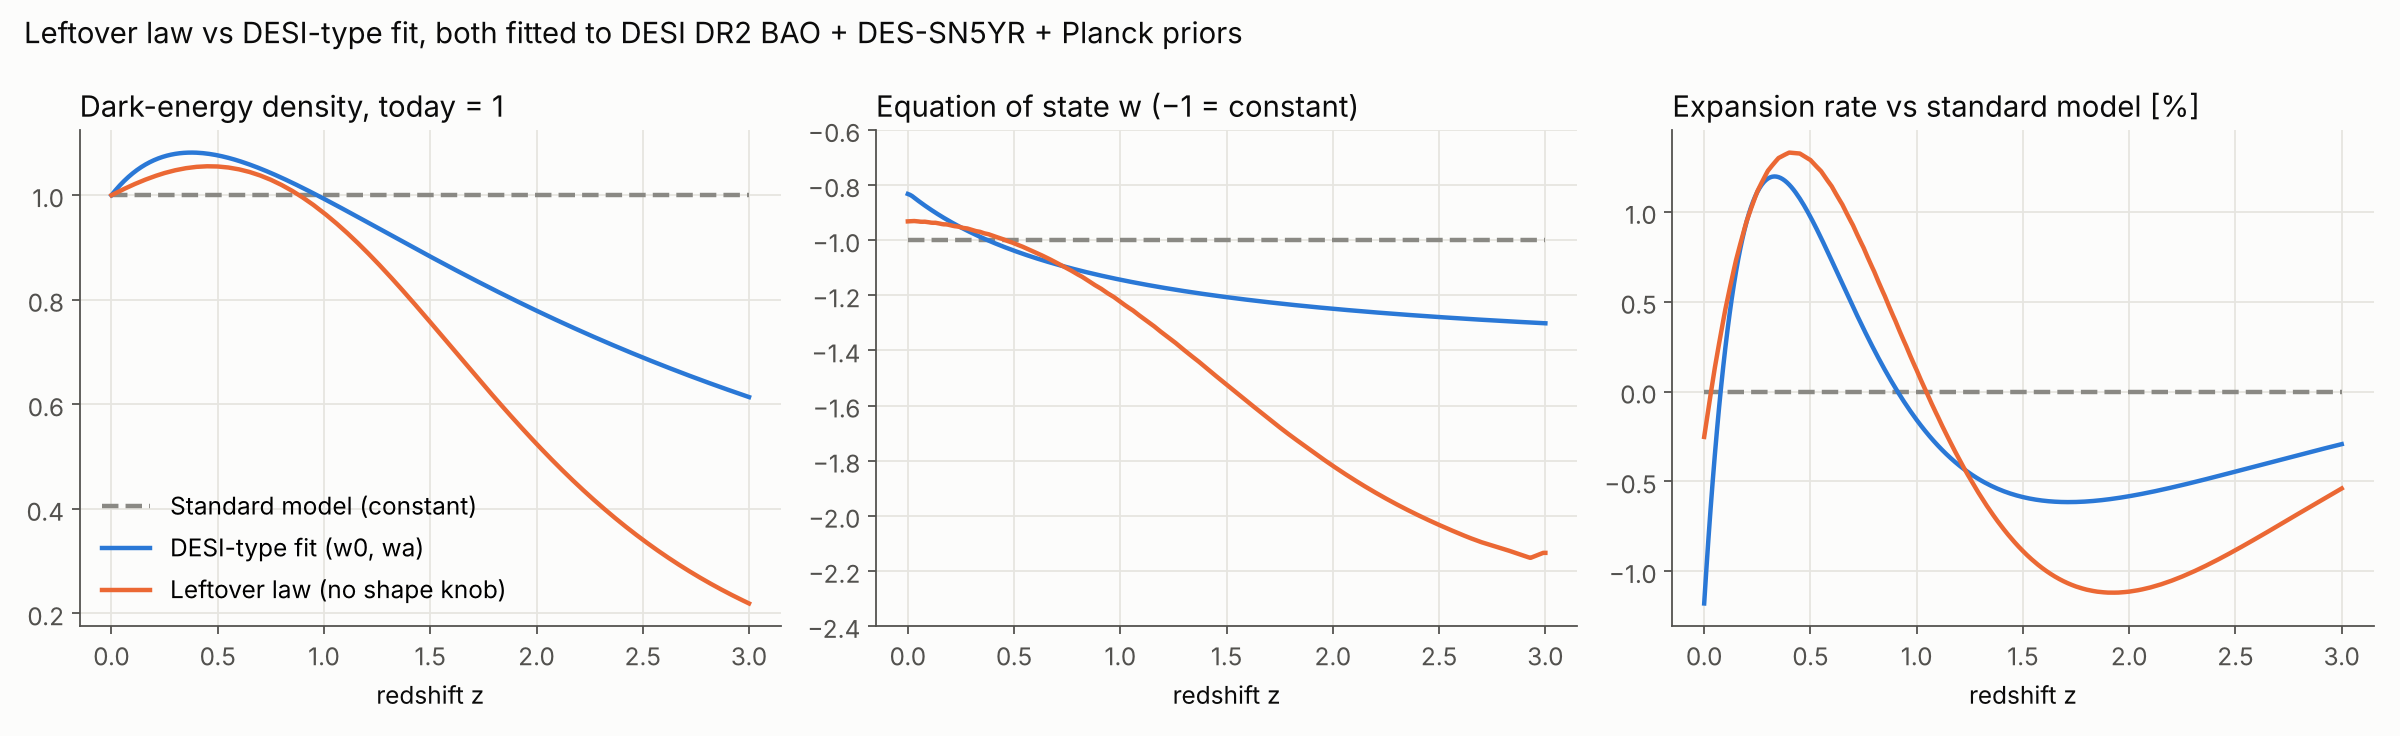
\includegraphics[width=\linewidth]{fig-de.png}
\caption{The leftover law (orange) and a DESI-type $w_0$--$w_a$ fit (blue), both fitted to DESI DR2 BAO, DES five-year supernovae and Planck
distance priors, against $\Lambda$CDM (dashed). Left: dark-energy density relative to today. Middle: equation of state. Right: expansion rate
relative to $\Lambda$CDM. The two agree below redshift 1 and part above 1.5.}\label{fig:de}
\end{figure}

\subsection{Predictions}
At the DES fit (Figure~\ref{fig:de}): dark energy peaks about 5--7\% above today near redshift 0.45--0.55, crosses $w=-1$ there, has
$w_0=-0.93$, and falls steeply before the peak, to 0.52 of today at $z=2$ and 0.40 at $z=2.33$, where DESI's form has 0.72. The expansion rate
is 1.3\% above $\Lambda$CDM at $z=0.5$ and 1.1\% below at $z=2$; against DESI's form the difference is about 0.5\% at $z\approx2$, while DESI DR2
measures $D_H$ at $z=2.33$ to 1.2\%. Growth runs 2.5--4.5\% above $\Lambda$CDM ($f\sigma_8$), and $S_8\approx0.85$ against 0.82, computed with CAMB
treating the term as smooth~\cite{camb}; that is 3.7$\sigma$ (5.2$\sigma$ without theory error) above DES six-year 3$\times$2pt in $\Lambda$CDM,
$0.789\pm0.012$, and 3.3$\sigma$ above its wCDM value, $0.782\pm0.021$~\cite{desy6} \chk{A15}. Two thirds of that rise comes from the higher matter density the data prefer, which DESI's form shares;
one third from the law itself (dark energy nearly absent before $z\approx2$ lets matter grow longer).

\paragraph{Limits of the fit.} The clumped share uses Press--Schechter grown at fixed $\Omega_m=0.31$, while the fits find 0.311--0.313 and
2.5--4.5\% more growth; the CMB enters as compressed distance priors; Union3 was not run; growth treats the term as smooth.

\paragraph{The amount.} Today's dark energy is $3.3$~keV/cm$^3$ and the supernova neutrinos made so far number about $3\times10^{-9}$/cm$^3$
\chk{A11}: each would have to make 1.1--3.4~TeV of dark energy. This window brackets $4\pi v=3.1$~TeV, the scale where the weak force's simple
description is expected to fail; a factor-three window near the weak scale catches many combinations, so this is numerology until derived.
Nothing in known physics ties a neutrino to a TeV of vacuum energy; the amount is the cosmological-constant problem itself.

\begin{erabox}
holds & Background only: the shape fits DESI DR2 + supernovae + Planck about as well as $w_0$--$w_a$ with no continuous knob (act and $M_{\rm esc}$ from a scan; 1--2$\sigma$ after trials); robust to the star-formation history; held-out tests pass but are not clean. \\
reading & Uncaptured leftovers of weak acts make room; clumping traps their sources; balanced relic baths do not drive. \\
open & $S_8$: 3.7--5$\sigma$ above DES lensing, and with lensing in, level with or behind $\Lambda$CDM; the amount; the field-equation form and its energy bookkeeping; an uneven (non-smooth) version. \\
test & $S_8$ and $f\sigma_8$ at $z=1$--1.5 (Euclid, Rubin, DESI full shape); $H$ at $z\ge1.5$ (full DESI, Euclid): a steep fall, not $w_0$--$w_a$'s slow one. \\
\end{erabox}

\section{The ledger}\label{sec:ledger}

Every item this stage tested, with its verdict: \textbf{H} holds, \textbf{R} reading, \textbf{X} refuted or dropped, \textbf{O} open.

{\small
\begin{longtable}{@{}rp{8.4cm}cp{4.6cm}@{}}
\toprule
\# & item & verdict & where \\
\midrule
\endhead
1 & Starobinsky inflation, does not fragment & H & \S\ref{sec:inflation}, our lattice \\
2 & Oscillons of the inflaton seed black-hole dark matter (v6) & X & \S\ref{sec:inflation} \\
3 & Information scalar as the fragmenting spectator & X & \S\ref{sec:inflation}, 60$\times$ short \\
4 & Rollout principle, with the time clause & R & \S\ref{sec:axioms} \\
5 & ``Slowest rollout'' as the speed of one switch & X & \S\ref{sec:switch}; holds as a sequence \\
6 & Switch = conformal dark U(1) bound into $B$ & R & \S\ref{sec:switch} \\
7 & Late patches are overdense & R & \S\ref{sec:switch}, qualitative, gauge dependent \\
8 & Black-hole dark matter with fast reheating & X & \S\ref{sec:bh}, gauge objection \\
9 & Black-hole dark matter with slow decay & O & \S\ref{sec:bh}, not excluded; $f=1$ by tuning $\beta/H$ to 9.5--14.6; dispersal caveat \\
10 & Asteroid window open & H & \S\ref{sec:bh} \\
11 & Hum below current limits, in future reach & H & \S\ref{sec:bh} \\
12 & One-event three-way test & O & \S\ref{sec:bh}; decisive only at $\sim10^{21}$~g; $f=1$ by construction \\
13 & Black holes make the matter surplus directly & X & \S\ref{sec:surplus} \\
14 & Cogenesis: dilution cancels in $\Omega_{\rm PBH}/\Omega_b$ & H & \S\ref{sec:surplus} \\
15 & Mirror preference $\epsilon\approx10^{-8}$ from the axioms & O & \S\ref{sec:surplus} \\
16 & Majorana neutrinos, seesaw at the switch scale & R & \S\ref{sec:neutrinos} \\
17 & Resonant pair or direct decay for $\epsilon$ & O & \S\ref{sec:neutrinos} \\
18 & Neutrino balance: normal ordering, sum 59.1~meV & R & \S\ref{sec:neutrinos}; sign chosen \\
19 & No $0\nu\beta\beta$ signal above $\sim4$~meV & O & \S\ref{sec:neutrinos}; a test \\
20 & Two independent witnesses leave a noise signature & X & Appendix~\ref{app:notes}; only if they differ \\
21 & Information scalar frozen before the electroweak split & R & \S\ref{sec:ew}, model consequence, no data \\
22 & $\alpha$ anywhere between 1 and 1/128 before the split & O & \S\ref{sec:ew}; clashes with running \\
23 & Lepton balance (Koide) & H & \S\ref{sec:ew}, 0.7\% \\
24 & Balance rules for quarks (695 other forms) & X & \S\ref{sec:ew}, at chance \\
25 & Georgi--Jarlskog near the switch era & R & \S\ref{sec:ew}, post hoc \\
26 & 3s1t sets the shape & R & \S\ref{sec:axioms}, restates Ehrenfest, Tegmark \\
27 & 3s1t sets the counts & X & \S\ref{sec:axioms}; the balance does \\
28 & $n^2-1$ counts; hypercharge as the balance mode & R & \S\ref{sec:ew} \\
29 & Confinement; first-order SU(3), smooth SU(2) & H & \S\ref{sec:hadrons}, lattice \\
30 & Glueball: mass from gluons alone & H & \S\ref{sec:hadrons}, lattice \\
31 & Vacuum energy lowest at $\theta=0$ & R & \S\ref{sec:hadrons}, reproduces Vafa--Witten \\
32 & Why nature sits at $\theta=0$ & O & \S\ref{sec:hadrons} \\
33 & $\eta'$ mass from the topological susceptibility & H & \S\ref{sec:hadrons}, $963\pm37$~MeV \\
34 & Pion as Goldstone ripple of the continuous balance & R & \S\ref{sec:hadrons}; the Goldstone pion holds on the lattice \\
35 & Continuum spin gap and $\Delta/N$ & H & \S\ref{sec:hadrons}, weak: linear-in-$a$ column only \\
36 & Witness rule gives the 56 baryon states & R & \S\ref{sec:hadrons}, = colour \\
37 & Opposite spins cheaper (spin balance) & R & \S\ref{sec:hadrons}, = hyperfine \\
38 & $\pi^0\to\gamma\gamma$ set by $\alpha^2$ & H & \S\ref{sec:hadrons}, 7.76 vs 7.8~eV; the ABJ anomaly \\
39 & Decays take the highest-entropy path & X & \S\ref{sec:hadrons}, handedness first \\
40 & $\pi^\pm-\pi^0$ from $\alpha$ & R & \S\ref{sec:hadrons}, 5.29 vs 4.59~MeV, 14\% high \\
41 & Quark--gluon plasma in oxygen collisions & R & \S\ref{sec:hadrons}, not discriminating \\
42 & Whole timeline passes reheating, BBN, CMB limits & H & \S\ref{sec:timeline} \\
43 & CMB tilt (ACT $n_s\approx0.974$) & O & \S\ref{sec:inflation}, external \\
44 & Information scalar as dark energy & X & \S\ref{sec:de} \\
45 & $4\pi$ mode-count rule with this timeline & X & \S\ref{sec:de} \\
46 & Deformed horizon entropy (Barrow, Tsallis) & X & \S\ref{sec:de} \\
47 & Acts spread evenly with matter & X & \S\ref{sec:de}, $+11$ to $+220$ \\
48 & Acts = fusion, or counted as conversions & X & \S\ref{sec:de} \\
49 & Relic neutrinos as drivers & X & \S\ref{sec:de}, $+262$ \\
50 & Leftover law: shape fits DESI + SN + CMB & H & \S\ref{sec:de}, background only; 1--2$\sigma$ after trials; with lensing level with $\Lambda$CDM \\
51 & Leftover law passes held-out tests & H & \S\ref{sec:de}; selection made on the full data \\
52 & $S_8\approx0.85$ against lensing & O & \S\ref{sec:de}, 3.7--5$\sigma$ (DES Y6, $\Lambda$CDM) \\
53 & The amount of dark energy & O & \S\ref{sec:de} \\
54 & Washout of the surplus by the Majorana $N$ ($K\sim50$) & O & \S\ref{sec:timeline}, not computed \\
\bottomrule
\end{longtable}}

\noindent Tally: 54 items; 13 hold, 15 are readings, 15 are refuted or dropped, 11 are open (after an independent review moved seven
verdicts from hold to reading or open and added item 54). Most of what holds is established physics the
timeline adopts or reproduces (Starobinsky, the gauge objection's rescue, lattice QCD); what is GUID's own is the order of the timeline,
the rollout principle, the lepton balance as a rule, and the dark-energy driver.

\section{Where it breaks}\label{sec:break}

\begin{enumerate}[leftmargin=*,itemsep=2pt]
\item \textbf{Growth.} The leftover law predicts $S_8\approx0.85$; DES's six-year lensing gives $0.789\pm0.012$ in $\Lambda$CDM and
$0.782\pm0.021$ in wCDM~\cite{desy6} (3.7--5$\sigma$ and 3.3$\sigma$ away), and HSC sources with DESI lenses $0.771^{+0.026}_{-0.027}$~\cite{porredon}.
Neither number is strictly valid for the law, since a 3$\times$2pt $S_8$ depends on the growth history assumed, but a rough prior already
cancels the law's background gain. If a full likelihood confirms this, the smooth law fails, unless an uneven version, made where acts
happen and stopped where matter clumps, slows growth inside clumps.
\item \textbf{The amount of dark energy} and \textbf{the mirror preference $\epsilon$}: two numbers the axioms do not supply. Without them the
dark-matter-to-matter ratio and today's acceleration are fitted, not predicted.
\item \textbf{The switch's speed.} $\beta/H$ is a free knob, and the black-hole abundance depends on it exponentially; the two matter-era
estimators differ by tens in $\ln P$, and the soft-profile thresholds are dispersal boundaries, not shown to end in black holes.
\item \textbf{Washout.} If the Majorana $N$ wash out the surplus during the switch's slow decay, the surplus needs $M_N$ well above
the maximum temperature, or another source.
\item \textbf{The CMB tilt.} If ACT's $n_s\approx0.974$ holds, Starobinsky as adopted is out at 2--3$\sigma$, and our matter era makes it worse.
\item \textbf{The hum.} If DECIGO or BBO hears nothing at 0.02--0.7~Hz at the predicted level, the slow-decay switch is not the source of
the dark matter.
\item \textbf{High-redshift expansion.} If the full DESI survey or Euclid finds dark energy fading slowly above redshift 1.5, as $w_0$--$w_a$ does,
rather than falling steeply, the leftover law fails.
\end{enumerate}

\section{Conclusion}

Read through DMP's axioms, one timeline holds together from the end of inflation to today: inflation adopted from physics, a hidden switch
that lags because its path has a barrier, black holes from the patches it leaves behind (not excluded as all of the dark matter, with a tuned speed), a hum and a matter surplus from the same event,
Majorana neutrinos, a lepton balance that beats chance, hadrons that a laptop lattice reproduces from gluons up, and a dark energy made by
the uncaptured leftovers of weak interactions and slowed as matter clumps. Each era names the measurement that can break it. Two numbers
are missing, the mirror preference and the amount of dark energy, and one prediction is in tension: the growth of structure, 3.7--5$\sigma$
above DES lensing, which with lensing included erases the law's edge over a constant. We claim
coherence where stated and failure where stated, not correctness. The first author's own words on what this is for: find where it fits,
where it breaks, and where it gets interesting.

\section*{Contributions and use of AI}
The first author set the direction, supplied every idea quoted with a time, and decided each fork (Starobinsky, dropping oscillons, the rollout
principle, Majorana, the dark-energy driver). Sirius, an AI coordinator (Claude, by Anthropic), translated the ideas into models, wrote and ran the
code in a cloud session and, through a remote session, on the first author's laptop, fitted the data and wrote this draft. A separate Claude session on
a separate plan ran the black-hole work package~\cite{wpbh}, and a further, independent Claude session reviewed the draft; its
findings (the lensing value, the fitting order, the trial count and seven verdicts) are applied here. Nothing here has been reviewed by a physicist.

\appendix
\section{The notes this paper is built from}\label{app:notes}
The working notes are kept with the first author; what they record that the paper uses is listed here. The runs behind every
quoted number are in this repository under \texttt{docs/guid-v7/runs/}, as they ran (their absolute paths are those of the session that ran them;
the survey data, DESI DR2 BAO, Pantheon+, DES-SN5YR and the LVK O3 spectrum, are public and not redistributed).
\begin{itemize}[leftmargin=*,itemsep=1pt]
\item \texttt{v7-notes-01-witness-noise-and-pbh-window.md}: the running log, 31~Oct--4~Nov. Its first section tests v6's hope that two
independent witnesses leave a statistical signature in noise: when both readings add, or a unanimity gate commits them, they do not (Gaussian
and Poisson sums stay single-source; the gate changes only the acceptance rate); only witnesses with different freshness times leave a
signature, and it is generic coloured noise (ledger item 20).
\item \texttt{v7-note-02-quarks-and-one-event.md}: the agreed timeline, the one-event table, the open list.
\item \texttt{v7-note-03-neutrinos-dirac-majorana.md}: the neutrino decision.
\item \texttt{v7-note-04-dark-energy.md} and \texttt{v7-de-prediction-card.md}: every dark-energy form, with its count.
\item \texttt{runs/bh/REPORT.md}: the black-hole work package (WP1--WP5).
\item \texttt{runs/pt/}: switch, cogenesis, timeline scripts and outputs; \texttt{runs/de/}: dark-energy fits and outputs. The balance fuzzing
and the lattice code are kept with the first author.
\item The lattice outputs and their summary, \texttt{FINAL\_continuum.txt}, on the first author's machine.
\end{itemize}
Run counts: 74 oscillon lattice runs (dropped route), 5 phase-transition lattice runs, about a dozen SU(3)/SU(2) pure-gauge jobs, quark runs at three
spacings (141, 208 and 100 configurations), 696 balance rules $\times$ 3 schemes $\times$ 20\,000 null universes, 62 dark-energy forms and 3 controls.

\section{The checks}\label{app:checks}
\texttt{checks.py} in this folder runs 60 checks: 37 re-derive analytic numbers from standard inputs (labelled A1--A15 in the text), 23 re-read
fitted numbers from the run outputs (labelled F). All 60 pass on 4~November 2026 (Python with numpy and scipy).

\begin{thebibliography}{99}\small
\bibitem{dmp} S.~Hrovat, \emph{Dark Matter Protocol (DMP)}, version 0.9.9, github.com/StevenHrovat/dmp (2026).
\bibitem{guidv6} S.~Hrovat and Sirius, \emph{GUID v6}, github.com/StevenHrovat/gravity, \texttt{docs/guid-v6/} (2026).
\bibitem{starobinsky} A.~A.~Starobinsky, Phys.\ Lett.\ B \textbf{91}, 99 (1980).
\bibitem{planck} Planck Collaboration, Astron.\ Astrophys.\ \textbf{641}, A10 (2020).
\bibitem{act} T.~Louis et al.\ (ACT), arXiv:2503.14452 (JCAP 2025); E.~Calabrese et al.\ (ACT), arXiv:2503.14454.
\bibitem{lozanov} K.~D.~Lozanov and M.~A.~Amin, Phys.\ Rev.\ D \textbf{97}, 023533 (2018), arXiv:1710.06851.
\bibitem{cotner2018} E.~Cotner, A.~Kusenko and V.~Takhistov, Phys.\ Rev.\ D \textbf{98}, 083513 (2018), arXiv:1801.03321.
\bibitem{ehrenfest} P.~Ehrenfest, Proc.\ Amsterdam Acad.\ \textbf{20}, 200 (1917).
\bibitem{tegmark} M.~Tegmark, Class.\ Quant.\ Grav.\ \textbf{14}, L69 (1997).
\bibitem{liu2021} J.~Liu, L.~Bian, R.-G.~Cai, Z.-K.~Guo and S.-J.~Wang, arXiv:2106.05637.
\bibitem{baker2021} M.~J.~Baker, M.~Breitbach, J.~Kopp and L.~Mittnacht, arXiv:2105.07481.
\bibitem{kawana} K.~Kawana and K.-P.~Xie, arXiv:2106.00111.
\bibitem{gouttenoire} Y.~Gouttenoire and T.~Volansky, arXiv:2305.04942.
\bibitem{lewicki} M.~Lewicki, P.~Toczek and V.~Vaskonen, arXiv:2305.04924.
\bibitem{aixie} W.-Y.~Ai and K.-P.~Xie, \emph{Reviving primordial black hole formation in slow first-order phase transitions}, arXiv:2605.11332 (v3).
\bibitem{franciolini} G.~Franciolini, Y.~Gouttenoire and R.~Jinno, Phys.\ Rev.\ Lett.\ \textbf{136}, 171404 (2026), arXiv:2503.01962.
\bibitem{confbound} arXiv:2506.15496, lower bound $\beta/H\sim5$ for conformal transitions (cited from our notes; not read).
\bibitem{escriva} A.~Escriv\`a, C.~Germani and R.~K.~Sheth, arXiv:1907.13311; arXiv:2007.05564.
\bibitem{harada2016} T.~Harada et al., arXiv:1609.01588.
\bibitem{gortongreen} M.~Gorton and A.~M.~Green, SciPost Phys.\ \textbf{17}, 032 (2024), arXiv:2403.03839.
\bibitem{wpbh} Black-hole work package, \texttt{docs/guid-v7/runs/bh/REPORT.md} (1~Nov 2026).
\bibitem{davidson} S.~Davidson and A.~Ibarra, Phys.\ Lett.\ B \textbf{535}, 25 (2002).
\bibitem{pilaftsis} A.~Pilaftsis and T.~E.~J.~Underwood, Nucl.\ Phys.\ B \textbf{692}, 303 (2004).
\bibitem{brannen} C.~A.~Brannen, \emph{The lepton masses}, APS Northwest Section meeting abstract and brannenworks.com/MASSES2.pdf (2006);
see also Y.~Koide, arXiv:hep-ph/0605074.
\bibitem{koide} Y.~Koide, Lett.\ Nuovo Cim.\ \textbf{34}, 201 (1982); Phys.\ Lett.\ B \textbf{120}, 161 (1983).
\bibitem{gj} H.~Georgi and C.~Jarlskog, Phys.\ Lett.\ B \textbf{86}, 297 (1979).
\bibitem{svetitsky} B.~Svetitsky and L.~G.~Yaffe, Nucl.\ Phys.\ B \textbf{210}, 423 (1982).
\bibitem{athenodorou} A.~Athenodorou and M.~Teper, JHEP \textbf{11}, 172 (2020), arXiv:2007.06422.
\bibitem{vafawitten} C.~Vafa and E.~Witten, Phys.\ Rev.\ Lett.\ \textbf{53}, 535 (1984).
\bibitem{witten} E.~Witten, Nucl.\ Phys.\ B \textbf{156}, 269 (1979).
\bibitem{veneziano} G.~Veneziano, Nucl.\ Phys.\ B \textbf{159}, 213 (1979).
\bibitem{greenberg} O.~W.~Greenberg, Phys.\ Rev.\ Lett.\ \textbf{13}, 598 (1964).
\bibitem{hannambu} M.~Y.~Han and Y.~Nambu, Phys.\ Rev.\ \textbf{139}, B1006 (1965).
\bibitem{das} T.~Das, G.~S.~Guralnik, V.~S.~Mathur, F.~E.~Low and J.~E.~Young, Phys.\ Rev.\ Lett.\ \textbf{18}, 759 (1967).
\bibitem{cmsoo} CMS Collaboration, Phys.\ Rev.\ Lett.\ \textbf{136}, 162301, arXiv:2510.09864.
\bibitem{desi} DESI Collaboration, DR2 Results II, arXiv:2503.14738.
\bibitem{padmanabhan} T.~Padmanabhan, arXiv:1206.4916 (2012).
\bibitem{madau} P.~Madau and M.~Dickinson, Ann.\ Rev.\ Astron.\ Astrophys.\ \textbf{52}, 415 (2014).
\bibitem{madaufragos} P.~Madau and T.~Fragos, Astrophys.\ J.\ \textbf{840}, 39 (2017).
\bibitem{ps} W.~H.~Press and P.~Schechter, Astrophys.\ J.\ \textbf{187}, 425 (1974).
\bibitem{bbks} J.~M.~Bardeen, J.~R.~Bond, N.~Kaiser and A.~S.~Szalay, Astrophys.\ J.\ \textbf{304}, 15 (1986).
\bibitem{pantheon} D.~Scolnic et al., Astrophys.\ J.\ \textbf{938}, 113 (2022); D.~Brout et al., ibid.\ \textbf{938}, 110 (2022).
\bibitem{desy5} DES Collaboration, DES-SN5YR with the Dovekie recalibration, github.com/des-science/DES-SN5YR (read 4~Nov 2026).
\bibitem{popovic} B.~Popovic et al., the Dovekie recalibration of DES-SN5YR, MNRAS (2026), arXiv:2511.07517 ($w_0=-0.803\pm0.054$, $w_a=-0.72\pm0.21$, 3.2$\sigma$).
\bibitem{chw} L.~Chen, Q.-G.~Huang and K.~Wang, JCAP \textbf{02}, 028 (2019), arXiv:1808.05724.
\bibitem{camb} A.~Lewis, A.~Challinor and A.~Lasenby, Astrophys.\ J.\ \textbf{538}, 473 (2000); CAMB 2.0.5.
\bibitem{desy6} DES Collaboration, Y6 3$\times$2pt, arXiv:2601.14559: $S_8=0.789\pm0.012$ ($\Lambda$CDM), $0.782\pm0.021$ (wCDM).
\bibitem{porredon} A.~Porredon et al., DESI-DR1 3$\times$2pt analysis, arXiv:2512.15960 (HSC-Y3 sources: $S_8=0.771^{+0.026}_{-0.027}$).
\end{thebibliography}
\end{document}
